\section{Writting}

LaTeX is a markup language, meaning that you write your document using commands and syntax that describe the structure and formatting of the document, rather than directly manipulating the visual appearance of the document as you would in a word processor. This allows for greater control and flexibility over the formatting of the document, but it also means that there is a learning curve to using LaTeX effectively.

In LaTeX, there is 2 main types of macros: commands and environments. Commands are used to perform specific actions, such as formatting text, inserting images, or creating tables. Environments are used to define a block of content that has a specific formatting or behavior, such as a section, a figure, or a table.

\subsection{Preamble}

The preamble of a \LaTeX document is the section that comes before the \texttt{\(\backslash\)begin\{document\}} command, and it is used to define the document class, load packages, and set up any custom commands or configurations for the document. The preamble is an important part of a \LaTeX document, as it allows you to customize the behavior and appearance of your document, and it can also help to ensure that your document is properly formatted and structured.

\subsection{Document management}

To structure your document, you can use sections, subsections, ... They follow this order:
  \begin{itemize}
    \item \texttt{\(\backslash\)part\{...\}} for parts
    \item \texttt{\(\backslash\)chapter\{...\}} for chapters (only in book and report document classes)
    \item \texttt{\(\backslash\)section\{...\}} for sections
    \item \texttt{\(\backslash\)subsection\{...\}} for subsections
    \item \texttt{\(\backslash\)subsubsection\{...\}} for subsubsections
    \item \texttt{\(\backslash\)paragraph\{...\}} for paragraphs
    \item \texttt{\(\backslash\)subparagraph\{...\}} for subparagraphs
  \end{itemize}

In addition, if you manage a multiple files document, you can use the \texttt{\(\backslash\)include} or \texttt{\(\backslash\)input} command to include the content of other files in your main document. The \texttt{\(\backslash\)include} command is used to include a file that contains a complete section or chapter of the document, while the \texttt{\(\backslash\)input} command is used to include a file that contains a smaller piece of content, such as a figure or a table. Both commands allow you to organize your document into multiple files, which can make it easier to manage and edit large documents.

\subsection{Text mode}

In text mode, you can write normal text, and use commands to format it. For example, the \texttt{\(\backslash\)textbf} command is used to make text bold, and the \texttt{\(\backslash\)emph} command is used to emphasize text (usually by italicizing it). You can also use commands to change the font size, color, or style of the text. The text mode is the default mode in LaTeX, and it is used for writing the main content of the document.

\subsection{Math mode}

In math mode, you can write mathematical expressions using a special syntax. For example, the \texttt{\(\backslash\)frac} command is used to create a fraction, and the \texttt{\(\backslash\)sum} command is used to create a summation symbol. Math mode also allows you to use special symbols and characters that are not available in text mode, such as Greek letters, operators, and delimiters. To enter math mode, you can use \texttt{\(\backslash\)(} and \texttt{\(\backslash\))} for inline math, or \texttt{\(\backslash\)[\(\backslash\)]} for display math, which is centered and on its own line.

\subsection{Commands}

Commands in LaTeX are defined using a backslash followed by the name of the command, and they can take arguments that specify the content or formatting of the command. For example, the \texttt{\(\backslash\)LaTeX} command is used to generate the LaTeX logo. Be aware that command can be mode specific, meaning that they can only be used in certain contexts or environments. For example, the \texttt{\(\backslash\)alpha} command is used to display the \(\alpha\) symbol, but it can only be used in math mode, which is a special environment for writing mathematical expressions.

\subsection{Environments}
Environments in LaTeX are defined using the \texttt{\(\backslash\)begin} and \texttt{\(\backslash\)end} commands, and they can also take arguments that specify the content or formatting of the environment. For example, the \texttt{itemize} environment is used to create a bulleted list, and it is defined as follows:
\begin{verbatim}
\begin{itemize}
  \item First item
  \item Second item
  \item Third item
  \item Fourth item
\end{itemize}
\end{verbatim}
This will generate a bulleted list with four items. The \texttt{itemize} environment can also be nested inside other environments, such as a section or a figure, to create more complex documents.

There is also math specific environments, such as the \texttt{equation} environment, which is used to create numbered equations, and the \texttt{align} environment, which is used to align multiple equations. These environments allow you to write complex mathematical expressions in a clear and organized way. Those enviroments are numbered by default, but you can add a \texttt{*} at the end of the environment name to create an unnumbered version of the environment, for example \texttt{equation*} and \texttt{align*}.

\subsection{Figure and tables}

Figure are also defined as environments, using the \texttt{figure} environment. Inside the figure environment, you can use the \texttt{\(\backslash\)includegraphics} command to include an image file, and you can also add a caption and a label to the figure for referencing it later in the document. For example:
\begin{verbatim}
\begin{figure}
  \centering
  \includegraphics[width=0.5\textwidth]{example-image}
  \caption{An example image}
  \label{fig:example}
\end{figure}
\end{verbatim}

Table are for their part defined using the \texttt{table} environment, and they can be created using the \texttt{tabular} environment inside the table environment. The \texttt{tabular} environment allows you to define the structure of the table, such as the number of columns and their alignment, and you can also add a caption and a label to the table for referencing it later in the document. For example:
\begin{verbatim}
\begin{table}
  \centering
  \begin{tabular}{|c|c|c|}
    \hline
    Column 1 & Column 2 & Column 3 \\
    \hline
    Data 1 & Data 2 & Data 3 \\
    Data 4 & Data 5 & Data 6 \\
    \hline
  \end{tabular}
  \caption{An example table}
  \label{tab:example}
\end{table}
\end{verbatim}
This will generate a table with three columns and two rows of data, with a caption and a label for referencing it later in the document. You can also customize the appearance of the table using various commands and packages, such as \texttt{booktabs} for creating professional-looking tables, or \texttt{tabularx} for creating tables with adjustable column widths. Math mode has also its own table environment, called \texttt{array}, which allows you to create tables with mathematical content, such as matrices or systems of equations. The syntax for the \texttt{array} environment is similar to the \texttt{tabular} environment, but it is designed specifically for mathematical content.

\subsection{Bibliography}

You can create a bibliography in LaTeX using the \texttt{thebibliography} environment, which allows you to list your references and cite them in the document. Inside the \texttt{thebibliography} environment, you can use the \texttt{\(\backslash\)bibitem} command to define each reference, and you can also use the \texttt{\(\backslash\)cite} command to cite the references in the text. For example:
\begin{verbatim}
\begin{thebibliography}{9}
  \bibitem{knuth} Donald E. Knuth. \textit{The TeXbook}. Addison-Wesley, 1984.
\end{thebibliography}
\cite{knuth}
\end{verbatim}

Or if you want you can use BibTeX or BibLaTeX, which are tools for managing bibliographies in LaTeX. They allow you to create a separate bibliography file (with a .bib extension) that contains all your references, and then you can use the \texttt{\(\backslash\)bibliography} command to include the bibliography in your document. This can make it easier to manage your references, especially if you have a large number of them, and it also allows you to easily switch between different citation styles using the \texttt{\(\backslash\)bibliographystyle} command.

\subsection{Cross-referencing}

You can create a cross-reference in LaTeX using the \texttt{\(\backslash\)label} and \texttt{\(\backslash\)ref} commands. The \texttt{\(\backslash\)label} command is used to define a label for a specific element in the document, such as a section, a figure, or a table, and the \texttt{\(\backslash\)ref} command is used to reference that label later in the document.

\subsection{Create figure and graphes}

The Tikz package is a powerful tool for creating high-quality graphics and diagrams in LaTeX. It allows you to create complex figures and graphs using a simple and intuitive syntax, and it provides a wide range of options for customizing the appearance of your graphics. With Tikz, you can create everything from simple shapes and lines to complex diagrams and plots, making it a versatile tool for creating visual content in your LaTeX documents.

For example, the following code draws two axes, a parabola and a point on it, and gives the Figure~\ref{fig:tikz}. This code is written in the file \texttt{src/TikZExample.tex}, which is used twice: once displayed as code with \texttt{\(\backslash\)verbatiminput}, and once compiled with \texttt{\(\backslash\)input}, so the figure always matches the code.
\verbatiminput{./../src/TikZExample.tex} % display the code of the file
\begin{figure}[h]
  \centering
  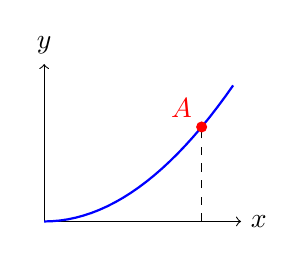
\begin{tikzpicture}
  \draw[->] (0,0) -- (2.5,0) node[right] {$x$};
  \draw[->] (0,0) -- (0,2) node[above] {$y$};
  \draw[blue, thick, domain=0:2.4]
    plot (\x, {0.3*\x*\x});
  \draw[dashed] (2,0) -- (2,1.2);
  \fill[red] (2,1.2) circle (2pt)
    node[above left] {$A$};
\end{tikzpicture}
 % compile the same file
  \caption{A simple TikZ drawing}
  \label{fig:tikz}
\end{figure}

\subsection{Create your own commands and environments}

You can create your own commands and environments in LaTeX using the \texttt{\(\backslash\)newcommand} and \texttt{\(\backslash\)newenvironment} commands. The \texttt{\(\backslash\)newcommand} command allows you to define a new command that can be used throughout your document, while the \texttt{\(\backslash\)newenvironment} command allows you to define a new environment that can be used to structure your document in a specific way. Creating your own commands and environments can help to simplify your document and make it easier to read and maintain, especially if you have complex formatting or repetitive content in your document. For example:
\begin{verbatim}
\newcommand{\R}{\mathbb{R}} % this will create a new command \R that will display the symbol for the set of real numbers
\newenvironment{myenv}{\begin{center}}{\end{center}} % this will create a new environment called myenv that will center the content inside it
\end{verbatim}

However, if you need to create more complex commands or environments, the \texttt{\(\backslash\)newcommand} and \texttt{\(\backslash\)newenvironment} commands may not be sufficient, and hard to use due on how they handle optional arguments. In this case, you can use the \texttt{\(\backslash\)NewDocumentCommand} and \texttt{\(\backslash\)NewDocumentEnvironment} commands from the \texttt{xparse} package, which provide more advanced features for creating custom commands and environments, such as support for optional arguments and more flexible syntax.
